\documentclass[11pt,a4paper]{article}
\author{TalentSprint}
\date{}
\usepackage{graphicx}
\usepackage{verbatim}
\usepackage{array}
\usepackage{caption}
\usepackage{enumitem}
\usepackage{xcolor}
\usepackage[tikz]{bclogo}
\usepackage{textcomp}
\usepackage{listings}
\usepackage{multicol}
\usepackage{float}
\usepackage{seqsplit} 
\usepackage{setspace}
\usepackage{soul}
\usepackage{latexsym}
\lstset{language=Java,numbers=left, numberstyle=\tiny, numbersep=10pt, showstringspaces=false, breaklines=true,keepspaces=true, columns=flexible}
\usepackage{fancyhdr}
\headheight=14pt
\lhead{\nouppercase{}}
\rhead{\nouppercase{\leftmark}}

\graphicspath{{../Images/}}


\begin{comment}
\setcounter{tocdepth}{1}
\setlength\parindent{0pt}
\parskip=4pt
\def\AnswerBox{\fbox{\begin{minipage}{4in}\hfill\vspace{0.5in}\end {minipage}}}

\thispagestyle{empty}
\vspace{1.5pc}
\topskip0pt
\vspace*{\fill}
\centerline{\sc \Huge Version Control System}
\vspace{2pc}
\vspace*{\fill}
\centerline{Prepared by TalentSprint WISE Team} 
\setcounter{page}{1}
\pagestyle{fancy}
\end{comment}


%========================================================================

% Lengths and widths
\addtolength{\textwidth}{2.5cm}
\addtolength{\hoffset}{0cm}
\setlength{\headsep}{-12pt} % Reduce space between header and content
\setlength{\headheight}{85pt} % If less, LaTeX automatically increases it
\renewcommand{\footrulewidth}{2pt} % Remove footer line
\renewcommand{\headrulewidth}{1pt} % Remove header line
\renewcommand{\seqinsert}{\ifmmode\allowbreak\else\-\fi} % Hyphens in seqsplit
% This two commands together give roughly
% the right line height in the tables
\renewcommand{\arraystretch}{1.3}
\onehalfspacing



% Commands
\newcommand{\SetRowColor}[1]{\noalign{\gdef\RowColorName{#1}}\rowcolor{\RowColorName}} % Shortcut for row colour
\newcommand{\mymulticolumn}[3]{\multicolumn{#1}{>{\columncolor{white}}#2}{#3}} % For coloured multi-cols
\newcolumntype{x}[1]{>{\raggedright}p{#1}} % New column types for ragged-right paragraph columns
\newcommand{\tn}{\tabularnewline} % Required as custom column type in use

% Font and Colours
\definecolor{HeadBackground}{HTML}{333333}
\definecolor{FootBackground}{HTML}{666666}
\definecolor{TextColor}{HTML}{333333}
\definecolor{DarkBackground}{HTML}{6B8E23} %{FD1AA8}
\definecolor{LightBackground}{HTML}{E8FED8} %D3FDC8
\definecolor{tit}{HTML}{FF6600}
\renewcommand{\familydefault}{\sfdefault}
\color{TextColor}
 \headsep = 25pt
% Header and Footer
\pagestyle{fancy}
\usepackage[headheight=110pt]{geometry}
\fancyhf{}% Clear header/footer

\fancyhead[r]{
\includegraphics[width = 4cm, height = 2cm]{TS-Logo.png}\hspace{0cm}}

%=================================TITLE=====================================
\fancyhead[l]{{\bf{\textcolor{tit}{\textrm{\large{Abstract Class, Interfaces and Wrapper Classes}}}}}}
%===========================================================================

\renewcommand{\headrulewidth}{0.4pt}% Default \headrulewidth is 0.4pt
\renewcommand{\footrulewidth}{0.4pt}% Default \footrulewidth is 0pt

\rfoot{Page \thepage}
\lfoot{COPYRIGHT \textcopyright TALENTSPRINT, 2015. ALL RIGHTS RESERVED.}



\begin{document}

\section*{Abstract Method and Abstract Class}
An abstract method does not contain any body. It contains only the method header, we can say it is an incomplete method. An abstract class is a class that generally contains some abstract methods. Both the abstract class and abstract methods should be declared by using the word `abstract'. Since abstract classes contains incomplete methods, it is not possible to estimate the total memory required to create the object. So, JVM cannot create objects to an abstract class. We should create sub classes and all the abstract methods should be implemented (body should be written) in the subclasses. Then, it is possible to create the object to the sub classes since they are complete classes.

\begin{lstlisting}[numbers=none]
abstract class ClassName {
    abstract methodName();
        concreteMethod(){}
}
\end{lstlisting}

Exaxmple, Let us write abstract class with an instance variable  \texttt{rate}, an abstract method \texttt{getRate()} and a concrete method \texttt{calculateBill()}
\begin{lstlisting}[numbers=none]
abstract class plan {
    protected double rate;
    public abstract void getRate();
    public void calculateBill(int units) {
        System.out.print(``BIll amount for ''+ units + ``units :'');
	System.out.println(rate*units);
    }
}
class CommercialPlan extends Plan {
    public void getRate() {
        rate = 5.00;
    }
}
class DomesticPlan extends Plan {
    public void getRate() {
	rate = 2.60;
    }
}
class Calculate {
    public static void main(String args[]) { 
	Plan p;
	System.out.println(``Commercial connection : '');
        p = new CommercialPlan();
	p.getRate();
	p.calculateBill(250);
        System.out.println(``Domestic connection: '');
        p = new DomesticPlan();
        p.getRate();
        p.calculateBill(150);
    }
}
\end{lstlisting}
\subsection*{Important Points}
\begin{itemize}
\item An abstract class is a class that contains 0 or more abstract methods.
\item An abstract class can contain instance variables and concrete methods in addition to abstact methods.
\item Abstract class and the abstract methods should be declared by using \texttt{`abstract'} keyword.
\item All the abstract methods of abstract class should be implemented in the sub class.
\item If any abstract method is not implemented, then that sub class should be declared as \texttt{`abstract'}. In this case, we cannot create object to the sub class. We should create another sub class and implement the remaining abstract method there.
\item We cannot create object to abstract class. But, we can create a reference of abstract class type.
\item The reference of abstract class can be used to refer to objects of its sub classes.
\item It is possible to derieve an abstract class as a sub class from a concrete super class.
\item We cannot declare a class both \lstinline!abstract! and \lstinline!final!.
\end{itemize}
\vfill{\ }
\begin{figure}[H]
 \begin{center}
   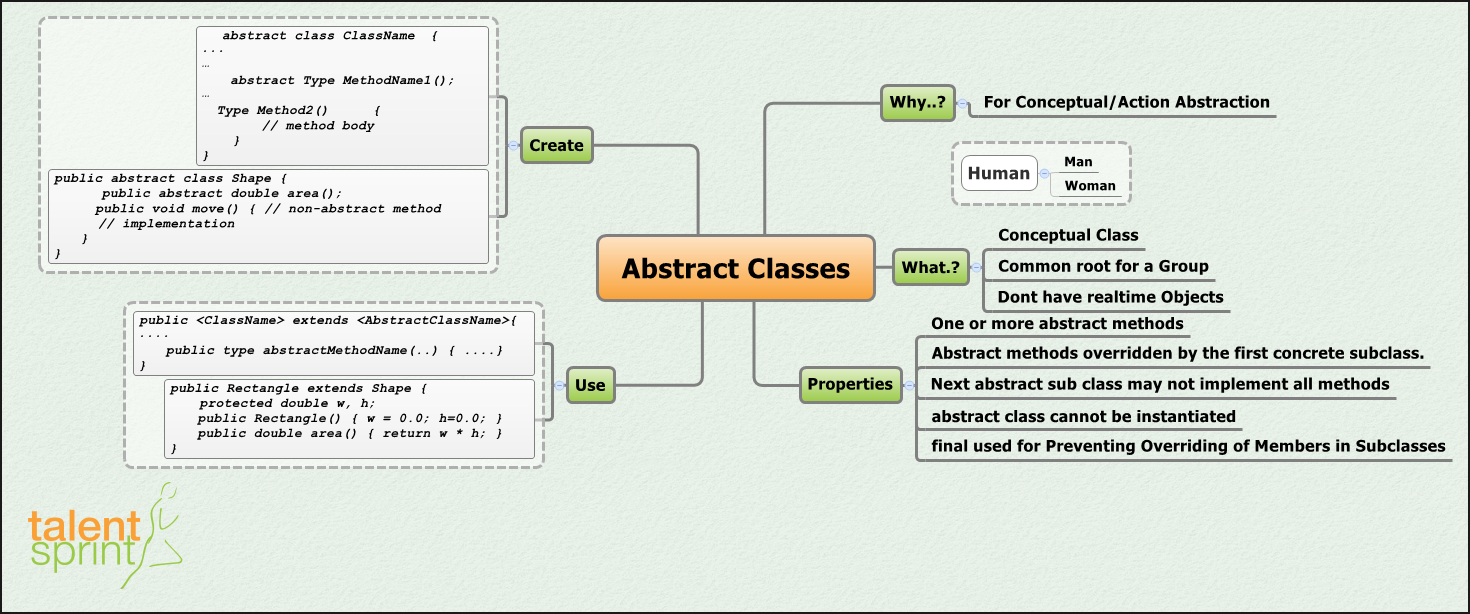
\includegraphics[angle=90,height=16cm, width=13cm]{AbstractClasses.png}
 \end{center}
 \end{figure}

\section*{Interface}
An interface contains only abstract methods which are all incomplete methods. It is not possible to create an object to an interface. In this case, we can create seperate classes where we can implement all the methods of the interface. These classes are called implementation classes. Since, implentation classes will have all the methods with body, it is possible to create objects to the implementation classes. The flexibility lies in the fact that every implementation class can have its own implementation of the abstract methods of the interface. 

\begin{lstlisting}[numbers=none]
    interface InterfaceName {
        variables;
        abstract methodName();
    }
\end{lstlisting}

Example, Write a program which contains a Printer interface and its implementation classes to send text to any printer.
\begin{lstlisting}[numbers=none]
impoert java.util.*;
interface Printer {
    void print(String text);
    void disconnect();
}
class IBMPrinter implements Printer {
    public void print(String text) {
        System.out.println(text);
    }
    public void disconnect() {
        System.out.println(``printing completed'');
        System.out.println(``Disconnected from IBM Printer'');
    }
}
class EpsonPrinter implements Printer {
    public void print(String text) {
        System.out.println(text);
    }
    public void disconnect() {
        System.out.println(``printing completed'');
        System.out.println(``Disconnected from Epson Printer'');
    }
}
class UsePrinter {
    public static void main(String args[]) {
        Scanner sc = new Scanner(System.in);
        System.out.println(``Enter the printer name'');
        String printername = sc.next();
        try {
            Class c = Class.forName(printername);
	    Printer ref = (Printer)c.newInstance();
            ref.print(``Hello, this is printed on the printer'');
            ref.disconnect();
       	}
	catch(Exception ref) {
            System.out.println(``Exception '' +ref);
        }
    }
}
\end{lstlisting}

\subsection*{Important Points}
\begin{itemize}
\item An interface is a specification of method prototypes. This means, only method names are written in the interface without method bodies.
\item An interface will have 0 or more abstract methods which are all public and abstract by default.
\item An interface can have variables which are public, static and final by default. This means all the variables of the interface are constants.
\item None of the methods in interface can be private, protected or static. 
\item We cannot create an object to an interface, but we can create a reference of interface type.
\item All the methods of interface should be implemented in its implementation classes. If any method is not implemented, then that implementation class should be declared as \texttt{`abstract'}
\item Interface reference can refer to the objects of its implementation classes.
\item When an interface is written, any third party vendor can provide implementation classes to it.
\item An interface can extend another interface.
\item An interface cannot implement another interface.
\item It is possible to write a class within an interface.
\item Interface forces the implementation classes to implement all of its methods compulsory. Java compiler checks whether all the methods are implemented in the implementation classes or not.
\item A class can implement (not extend) multiple interfaces. 
\begin{lstlisting}[numbers=none]
    class MyClass implements Interface1, Interface2 
    class MyClass extends Class1 implements Interface1, Interface2
\end{lstlisting}
\end{itemize}
\section*{Multiple Inheritance Using Interfaces}
In multiple inheritance, sub classes are derived from multiple super classes. If two super classes have same name for their class members (variables and methods) then which member is inherited into the sub class is the main confusion in multiple inheritance. This is the reason, Java does not support the concept of multiple inheritance. This confusion is reduced by using mutiple interfaces to achieve multiple inheritance. For exmaple

\begin{lstlisting}[numbers=none]
    interface Interface1 {
        int x = 20; // public static final
        void method(); // public abstract
    }
    interface Interface2 {
        int x = 30;
        void method();
    }
\end{lstlisting}
And there is an implementation class MyClass as :

\begin{lstlisting}[numbers=none]
    class MyClass implements Interface1, Interface2 
\end{lstlisting}

Now there is no confusion to refer to any of the members of the interfaces from MyClass. For example, to refer to interface Interface1 and Interface2 we can write :
\begin{lstlisting}[numbers=none]
    Interface1.x
    Interface2.x
\end{lstlisting}

Similarly there will not be any confusion regarding which method is available to the implementation class.

\textbf{Example} Write a program to illustrate how to achieve multiple inheritance using multiple interfaces.

\begin{lstlisting}[numbers=none]
interface Father {
    float ht = 6.2f;
    void height();
}
interface Mother {
    float ht = 5.8f;
    void height();
}
class child implements Father, Mother {
    public void height() {
        float ht = (Father.ht + Mother.ht) / 2;
        System.out.println(``Child's height '' +ht);
    }
}
class MultipleInheritance {
    public static void main(String args[]) {
        child ch = new child();
        ch.height();
    }
}
\end{lstlisting}
\begin{figure}[H]
 \begin{center}
   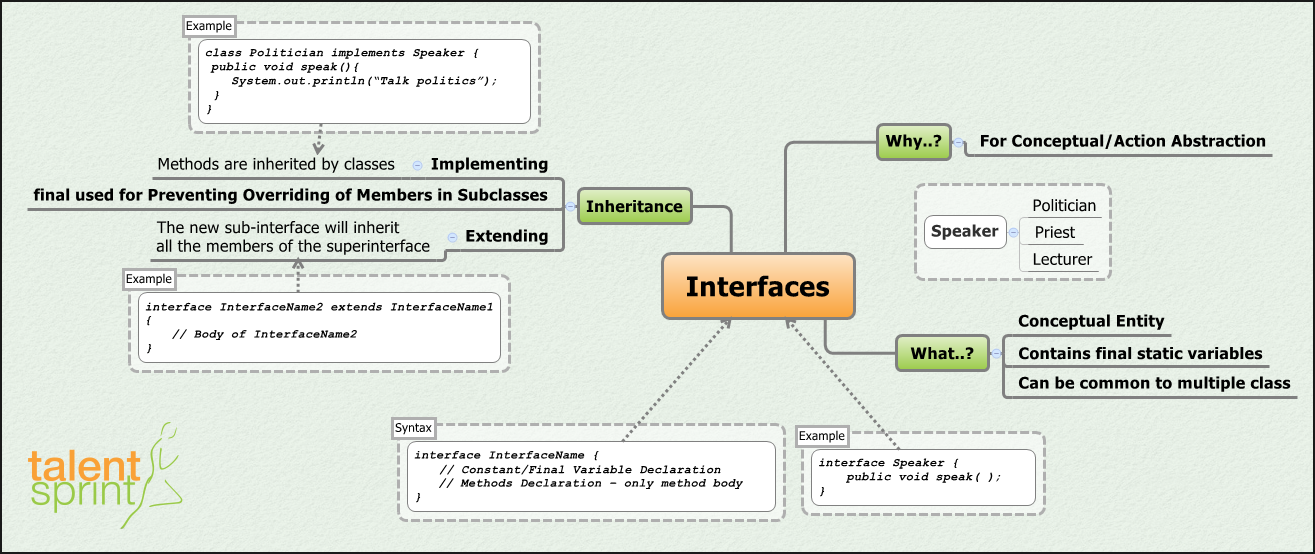
\includegraphics[angle=90,height=20cm, width=13cm]{Interfaces.png}
 \end{center}
 \end{figure}

 \section*{Wrapper Classes}
Wrapper classes are used to convert any data type into an object. The primitive data types are not objects; they do not belong to any class; they are defined in the language itself. Sometimes, it is required to convert data types into objects in Java language. Each of Java's eight primitive data types has a class dedicated to it. These are known as wrapper classes, because they ``wrap'' the primitive data type into an object of that class. The wrapper classes are part of the java.lang package, which is imported by default into all Java programs.
\begin{description}  
\item [Integer] is a wrapper class of the primitive \emph{int}
\item [Character] is a wrapper class of the primitive \emph{char}
\item [Double] is a wrapper class of the primitive \emph{double}
\end{description}

\subsubsection*{Converting Primitive Types to Objects (Wrapper) and the vise versa}
\begin{table}[H]
\centering
\begin{tabular}{|p{2.5 cm}|p{4 cm}|p{6 cm}|}  \hline

%\multicolumn{3}{|c|}{\textbf{Attributes}}\\\hline
\multicolumn{1}{|c|}{\textbf{Primitive type} } & \multicolumn{1}{|c|}{\textbf{Primitive to Object}} & \multicolumn{1}{|c|}{\textbf{Object to Primitive}} \\\hline
 double d = 5.0; &Double aDouble = new Double(d);&double r = aDouble.doubleValue();\\ \hline
 int i = 5 &Integer dataCount = new Integer(i); &int newCount = dataCount.intValue(); \\ \hline
 \end{tabular}
\end{table}

A common translation you need in programs is converting a \lstinline!String! to a numeric type, such as an \lstinline!int! (Object --\textgreater  primitive).
\begin{lstlisting}[numbers=none]
 String pennsylvania = "65000";
 int penn = Integer.parseInt(pennsylvania);
\end{lstlisting}
\vfill{\ }

\subsubsection*{Primitive Types and their Wrapper Classes}
The following table lists the primitive types and the corresponding wrapper classes:

\begin{table}[H]
\centering
\begin{tabular}{|p{3 cm}|p{5.5 cm}|}  \hline

%\multicolumn{3}{|c|}{\textbf{Attributes}}\\\hline
\multicolumn{1}{|c|}{\textbf{Primitive type} } & \multicolumn{1}{|c|}{\textbf{Wrapper Class}} \\\hline
boolean & java.lang.Boolean \\ \hline
byte & java.lang.Byte \\ \hline
char & java.lang.Character \\ \hline
double & java.lang.Double \\ \hline
float & java.lang.Float \\ \hline
int & java.lang.Integer \\ \hline
long & java.lang.Long \\ \hline
short & java.lang.Short \\ \hline
void & java.lang.Void \\ \hline
 \end{tabular}
\end{table}


\subsubsection*{Converting Primitive Types to Strings}
\begin{description}
\item [valueOf()] method of \emph{\textbf{String}} class is used to convert numerical values to strings.
\begin{lstlisting}[numbers=none]
int i = 1;
double d = 5.0;
String dStr = String.valueOf(d);
String iStr = String.valueOf(i);
\end{lstlisting}
\end{description}



\end{document}